Extensive research on HER flooded journals over the past decade, as well as numerous online competitions hosted in the last couple of years. There are now several unimodal models that are extremely successful in identifying human expressions using pictures of faces, body position, physiological signal data, as well as audio clips. The variety of ways to recognize human emotions are summarized in Figure \ref{fig:tree}. A majority of HER research is focused on nonverbal communication following psychologists claims that nonverbal communication is overpowering in conversation and establishes the most important means of portraying emotions \cite{mehrabian-1971}\cite{ekman-1992} and that a facial expression is the primary predictor of emotion \cite{plutchik-2001}\cite{darwin-1896}. 

\begin{figure}[ht]
\begin{center}
    {\footnotesize
    \begin{forest}
        for tree={%
            edge path={\noexpand\path[\forestoption{edge}] (\forestOve{\forestove{@parent}}{name}.parent anchor) -- +(0,-10pt)-| (\forestove{name}.child anchor)\forestoption{edge label};}, s sep=1.5mm, inner sep=1, l=0  
        }
        [
        \underline{Human Emotion Recognition}
            [Non-Verbal Communication
                [Face]
                [Body]
                [Physiological]
            ]
            [Verbal Communication
                [Speech]
                [Text]
            ]
        ]
    \end{forest}
    }
\end{center}
\caption{Human Emotion Recognition Modalities}\label{fig:tree}
\end{figure}

Often times facial expressions are not available and other modalities are required to understand emotions. Body gestures, physiological data provided by wearable devices, and speech can also be used in an attempt to recognize emotions.


\subsection{Facial Expression Recognition}
    Notable psychologists deduced the most basic human emotions using facial expressions as their primary means of analysis \cite{plutchik-2001}\cite{ekman-1992}\cite{darwin-1896}. Needless to say, facial expressions are one of the most important pieces of the HER puzzle. As such, FER has piqued the interest of researchers and data analysis competitions around the world. 
    
    Several decades were spent finding and analyzing the best features to include to yield the best prediction accuracy in a traditional or classical machine learning model. However, with the rapid development of deep learning machines, coupled with the discovery of Convolutional Neural Networks (CNN) and Transformers, recent approaches to FER capitalize on the advantages of DL to achieve the highest prediction accuracy of expressed emotion given a facial expression. The trends through mid-2019 of classical approaches compared to neural network based approaches is visualized in Figure \ref{fig:trad_vs_nn}.
        
    \begin{figure}[!htb]
    \centering
    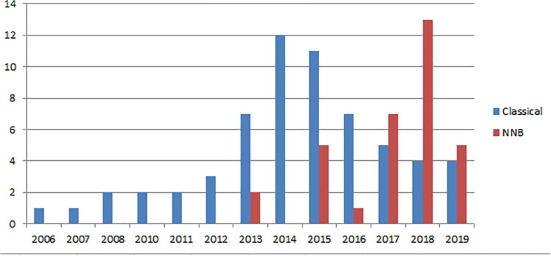
\includegraphics[width=.5\textwidth]{figures/trad_vs_nn.jpg}
    \caption{\label{fig:trad_vs_nn} Classical vs. Neural Network Based Approaches to Facial Expression Recognition \cite{canal-2022}}
    \end{figure} 

     Common FER datasets contain images or videos of facial expressions where either 6, 7 or 8 distinct emotion categories are labeled. The most popular dataset in the last two years is AffectNet \cite{mollahosseini_affectnet_2019} which contains around 0.4 million images labeled with one of eight facial expressions including the intensity of valence and arousal lending itself useful for both categorical and dimensional emotion models. A small subset of these images are shown in Figure \ref{fig:fer}. In order to better represent candid facial expressions instead of over-expressive ones found in other datasets, the Acted Facial Expressions in the Wild (AFEW) database was created \cite{dhall}. There are several other databases like the Japanese Female Facial Expression (JAFFE) \cite{lyons} and the Cohn-Kanade extended database (CK+) \cite{lucey} that contain well-labeled images of facial expressions, however they are less representative of the real world when compared to AffectNet and AFEW. 
    
    \begin{figure}[!htb]
    \centering
    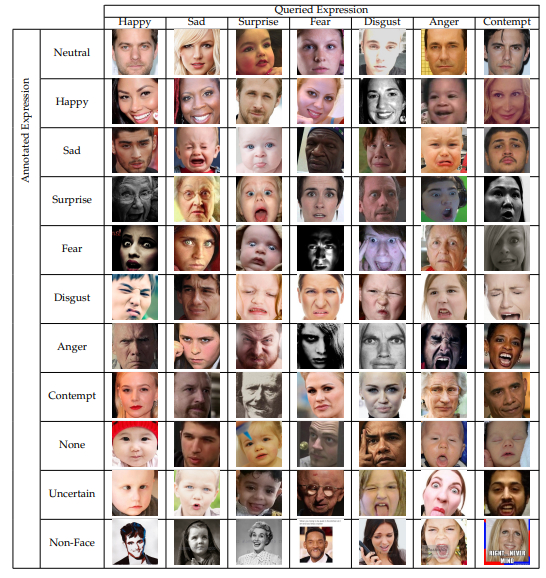
\includegraphics[width=.3\textwidth]{figures/faces.png}
    \caption{\label{fig:fer} AffectNet Database of Facial Expressions \cite{mollahosseini_affectnet_2019}}
    \end{figure}

    \begin{table}[ht]
        \centering
        \begin{tabular}{|p{0.16\linewidth}|p{0.27\linewidth}|p{0.21\linewidth}|p{0.12\linewidth}|}
        \hline
        Database & Author & Model & Accuracy\\\hline
        
        AffectNet (7 emotions)
        & Antoniadis et al. \cite{antoniadis_exploiting_2021}
        & Emotion-GCN
        & 66.46\%\\\hline
        
        AffectNet (8 emotions)
        & Savchenko et al. \cite{savchenko-2022}
        & Multi-task EfficientNet-B2
        & 63.03\%\\\hline

        AFEW
        & Savchenko et al. \cite{savchenko-2022}
        & Multi-task EfficientNet-B0
        & 59.27\%\\\hline
        
        CK+
        & Aouayeb et al. \cite{aouayeb-2021}
        & ViT + SE
        & 99.80\%\\\hline

        JAFFE
        & Aouayeb et al. \cite{aouayeb-2021}
        & ViT + SE
        & 94.83\%\\\hline
        
        \end{tabular}
        \caption{\label{tab:speech}Speech Emotion Recognition Models.}
    \end{table}

    Antoniadis et al. \cite{antoniadis_exploiting_2021} proposes a Graph Convolutional Network (GCN) model that includes both the categorical model (7 emotions) and two dimensional model (valence and arousal). The GCN encapsulates the dependencies between both the facial expression classifiers and the valence-arousal regressors. This approach achieved 66.46\% prediction accuracy for 7 emotion classifiers on AffectNet. 
    
    Savchenko et al. \cite{savchenko-2022} creates two CNNs that achieve 63.03\% (EfficientNet-B2) on AffectNet when classifying 8 emotions and 59.27\% (EfficientNet-B0) on AFEW. Their models build on previous lightweight, robust FER CNN models for face recognition and the fine-tuned their model on emotion classification. They novel contribution of this research is a modified CNN optimizer. The constructed CNN wass then used to predict the emotion classifier using AffectNet and AFEW.
    
    Zhang et al. \cite{zhang_2022} recognizes the existance of noisey samples in FER datasets and proposes a novel Erasing Attention Consistency (EAC) method to reduce the effects of these noisy samples during CNN model training. This approach resulted in 65.32\% prediction accuracy on AffectNet. 
    
    Aouayeb et al. \cite{aouayeb-2021} leverages a recently successful approach to computer vision called a vision transformer. This transformer is used to extract smaller  features of the facial expression. The second part of the their approach employs a Squeeze and Excitation block to extract meaning from these smaller features to classify the emotion expressed in the image. This model was applied to multiple datasets, but the most noteworthy achievements are the accuracy for the CK+ and JAFFE datasets of 99.8\% and 94.83\%, respectively.    

    Datasets like JAFFE and CK+ have promising near-perfect results, but these datasets have an extremely small number of images with a very small number of unique subjects. Not only does AffectNet contain 0.4 million facial expressions, it also contains images from different angles, with different shadowing, various skin tones, and subjects of a wide variety of ages, making it more representative of the real world and thus more challenging to predict emotions. Additionally, AffectNet is cited in almost double the number of papers in comparison to other smaller datasets. Despite the surge in performance of models applied to these datasets, the best models applied to AffectNet are still only achieving around 63\% accuracy \cite{savchenko-2022} to classify 8 emotions and 66.5\% to classify 7 emotions \cite{antoniadis_exploiting_2021}. This is clear evidence that standalone facial expressions will not be a sufficient approach to recognize human emotions. 


\subsection{Body Movement (Gesture) Recognition}
    Although facial expressions dominate a majority of nonverbal communication, body movement and gestures can also contribute to nonverbal communication. This component is commonly known as body language and is depicted in Figure \ref{fig:body}. Research on body language is very broad as a result of the various ways humans use body language to communicate. Humans use hand gestures, eye movement and touch to communicate emotions which makes databases more difficult to create, as well as models' prediction accuracy. A majority of body language research utilizes an ensemble of body parts or a kinematic model shown in Figure \ref{fig:gesture-recognition}. Using these models of the human body, body pose estimation can be used to help recognize the emotion that is being expressed \cite{noroozi-2021}.   
    
    \begin{figure}[!htb]
    \centering
    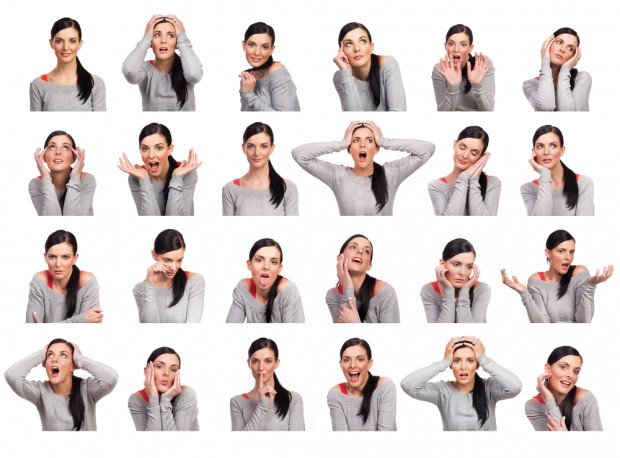
\includegraphics[width=.3\textwidth]{figures/bodylanguage.png}
    \caption{\label{fig:body} Body Language Expressions \cite{noroozi-2021}}
    \end{figure} 
    
    \begin{figure}[!htb]
    \centering
    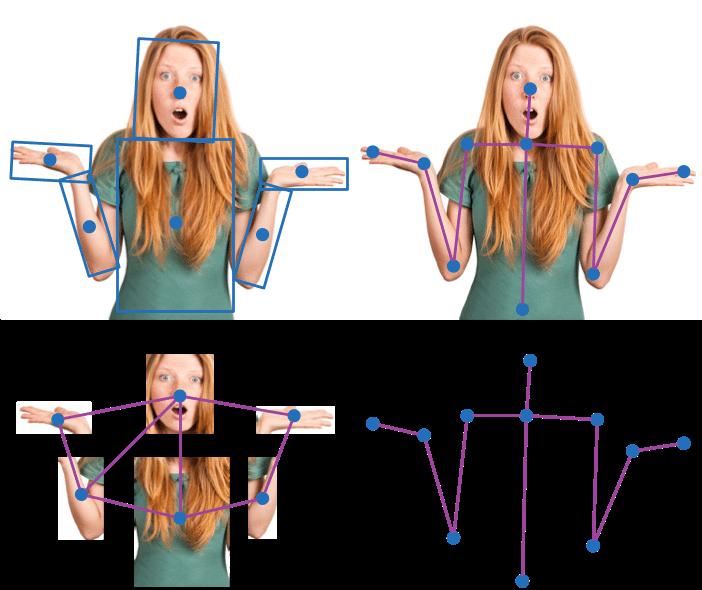
\includegraphics[width=.3\textwidth]{figures/gesture_recognition.jpg}
    \caption{\label{fig:gesture-recognition} Gesture Recognition - Ensemble of Body Parts (left) and Kinematic Model (right) \cite{noroozi-2021}}
    \end{figure} 


\subsection{Physiological Signal Processing}
    With the availability and popularity of smart watches, fitness bands and other wearable computing devices, the access to basic physiological data greatly increased. Interest in the link between emotions and physiological data, however, did not start there. Psychologists have always been keen on categorizing emotions and what constitutes one emotion compared to another. Emotion recognition is popular using electroencephalograph (EEG), electrocardiogram (ECG), and/or electrodermal activity (EDA) databases \cite{xiao-2022}. There are several datasets that contain all three of these physiological signals (BIO-VID-EMO DB being the biggest) that collect physiological data when the subject is watching a movie clip specifically selected to evoke an emotional response. The BIO-VID-EMO database \cite{zhang_biovid_2016} contains labels for valence, arousal, and five different emotions. 


\subsection{Speech Emotion Recognition}
    Another avenue for humans to communicate their emotions is through speech. The content of words someone speaks, coupled with the pitch and tone of their voice, contain a multitude of information that can describe their emotional state. The primary tool for leading research of SER is a type, or combination of types, of neural networks. Table \ref{tab:speech} summarizes the leading models for each dataset.

    Three of the most popular databases are the Berlin Emotional Database \cite{noauthor_emo-db_nodate} (Emo-DB), the Interactive Emotional Dyadic Motion Capture (IEMOCAP) database \cite{busso_iemocap_2008}, and the Ryerson Audio-Visual Database of Emotional Speech and Song (RAVDESS) \cite{livingstone_ryerson_2018}. Emo-DB contains 500 audio clips of words labeled by seven different emotions. The IEMOCAP dataset is more complex and can be used in mutlimodal models because the dataset contains 302 recorded videos annotated for the presence of nine emotions, as well as valence, arousal and dominance. Similar to IEMOCAP, but less used, RAVDESS is a large database comprises 7356 files containing 24 professional actors (12 female and 12 male) speaking various statements and expressing one of eight emotions, as well as singing and expressing one of six emotions. Each expression is also labeled according to its intensity of normal or strong.

    Ye et al. \cite{ye_temporal_2022} propose a temporal-aware network bi-directional multi-scale network (TIM-Net) which learns emotions from different time scales and then integrates additional information from different time periods for context and finally combines all this information back together to make a prediction on the emotion displayed. This model was tested and performed well on several benchmark datasets: IEMOCAP, RAVDESS, EmoDB, EMOVO \cite{costantini2014emovo} and SAVEE \cite{jackson}. This dominating model attained these respective accuracies when tested on each dataset: 71.65\%, 92.08\%, 95.7\%, 92\%, and 87.71.   

    Lian et al. \cite{lian-2020} employs a domain adversarial neural network (DANN) and incorporates context information for emotion recognition. This research explains the fusion of audio and text data and a self-attention based gated recurrent unit for contextual feature extraction on the IEMOCAP database and achieved the highest weighted accuracy on this dataset with 82.7\%.

    Wagner et al. \cite{wagner-2022} utilizes the first transformer-based architecture for dimensional speech emotion recognition to predict the level of valence, arousal, and dominance using the MSP-Podcast dataset \cite{martinez} and IEMOCAP. This models achieves a concordance correlation coefficient of 0.638 (valence), 0.745 (activation), and 0.655 (dominance) on the MSP-Podcast dataset.

    \begin{table}[ht]
        \centering
        \begin{tabular}{|p{0.15\linewidth}|p{0.2\linewidth}|p{0.15\linewidth}|p{0.15\linewidth}|}
        \hline
        Database & Author & Model & Accuracy\\\hline
        
        IEMOCAP
        & Lian et al. \cite{lian-2020}
        & Context-Dependent DANN
        & 82.7\%\\\hline
        
        RAVDESS
        & Ye et al. \cite{ye_temporal_2022}
        & TIM-Net
        & 92.08\%\\\hline
        
        Emo-DB
        & Ye et al. \cite{ye_temporal_2022}
        & TIM-Net
        & 95.7\%\\\hline
        
        EMOVO
        & Ye et al. \cite{ye_temporal_2022}
        & TIM-Net
        & 92\%\\\hline

        SAVEE
        & Ye et al. \cite{ye_temporal_2022}
        & TIM-Net
        & 97.71\%\\\hline
        
        \end{tabular}
        \caption{\label{tab:speech}Speech Emotion Recognition Models.}
    \end{table}
